\documentclass[11pt]{article}

\usepackage[a4paper,margin=1in]{geometry}
\usepackage{amsmath,amssymb,amsfonts}
\usepackage{tikz}
\usetikzlibrary{positioning,arrows.meta,calc}
\usetikzlibrary{positioning}

\begin{document}
	
	\section*{Adding Noise to the Input}
	
	For a simple linear output neural network, adding Gaussian noise to the
	input is equivalent to adding an $L_2$ penalty (weight decay) on the
	weights.
	
	It can also be interpreted as a form of data augmentation.
	
	\vspace{1cm}
	
	%%%%%%%%%%%%%%%%%%%%%%%%%%%%%%%%%%%%%%%%%%%%%%%%%%%%%%%%%%%%%%
	\subsection*{Input Noise Model}
	
	\begin{center}
		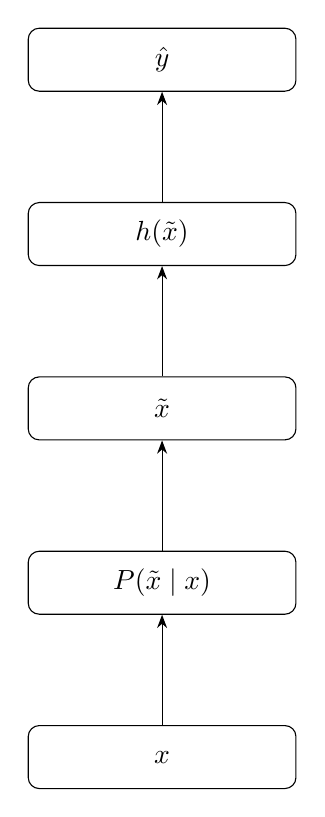
\begin{tikzpicture}[
			node distance=1.4cm,
			block/.style={draw,rounded corners,minimum width=3.4cm,minimum height=0.8cm},
			>=Stealth
			]
			
			\node[block] (x) {$x$};
			
			\node[block,above=of x] (noise)
			{$P(\tilde{x}\mid x)$};
			
			\node[block,above=of noise] (xtilde)
			{$\tilde{x}$};
			
			\node[block,above=of xtilde] (net)
			{$h(\tilde{x})$};
			
			\node[block,above=of net] (y)
			{$\hat{y}$};
			
			\draw[->] (x)--(noise);
			\draw[->] (noise)--(xtilde);
			\draw[->] (xtilde)--(net);
			\draw[->] (net)--(y);
			
		\end{tikzpicture}
	\end{center}
	
	%%%%%%%%%%%%%%%%%%%%%%%%%%%%%%%%%%%%%%%%%%%%%%%%%%%%%%%%%%%%%%
	\subsection*{Single Output Neuron}
	
	\begin{center}
		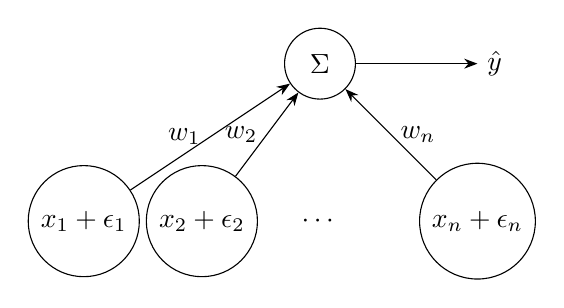
\begin{tikzpicture}[>=Stealth]
			
			\node[circle,draw,minimum size=9mm] (n) at (0,0) {$\Sigma$};
			
			\node[circle,draw] (x1) at (-3,-2) {$x_1+\epsilon_1$};
			\node[circle,draw] (x2) at (-1.5,-2) {$x_2+\epsilon_2$};
			\node (dots) at (0,-2) {$\cdots$};
			\node[circle,draw] (xn) at (2,-2) {$x_n+\epsilon_n$};
			
			\draw[->] (x1)--node[left] {$w_1$}(n);
			\draw[->] (x2)--node[left] {$w_2$}(n);
			\draw[->] (xn)--node[right] {$w_n$}(n);
			
			\draw[->] (n)--++(2,0) node[right] {$\hat{y}$};
			
		\end{tikzpicture}
	\end{center}
	
	Each input is corrupted by independent Gaussian noise,
	
	\[
	\epsilon_i \sim \mathcal{N}(0,\sigma^2),
	\]
	
	therefore
	
	\[
	\tilde{x}_i=x_i+\epsilon_i.
	\]
	
	The clean network output is
	
	\[
	\hat{y}=\sum_{i=1}^{n}w_ix_i.
	\]
	
	The noisy output becomes
	
	\[
	\tilde{y}
	=
	\sum_{i=1}^{n}w_i\tilde{x}_i
	=
	\sum_{i=1}^{n}w_i(x_i+\epsilon_i).
	\]
	
	Hence,
	
	\[
	\tilde{y}
	=
	\hat{y}
	+
	\sum_{i=1}^{n}w_i\epsilon_i.
	\]
	
	%%%%%%%%%%%%%%%%%%%%%%%%%%%%%%%%%%%%%%%%%%%%%%%%%%%%%%%%%%%%%%
	\subsection*{Expected Squared Error}
	
	We are interested in
	
	\[
	E[(\tilde{y}-y)^2].
	\]
	
	Substituting $\tilde{y}$,
	
	\[
	E\left[
	\left(
	(\hat{y}-y)
	+
	\sum_{i=1}^{n}w_i\epsilon_i
	\right)^2
	\right].
	\]
	
	Expanding,
	
	\[
	=
	E[(\hat{y}-y)^2]
	+
	2E\left[
	(\hat{y}-y)
	\sum_{i=1}^{n}w_i\epsilon_i
	\right]
	+
	E\left[
	\left(
	\sum_{i=1}^{n}w_i\epsilon_i
	\right)^2
	\right].
	\]
	
	Since
	
	\[
	E[\epsilon_i]=0,
	\]
	
	and the noise is independent of $(\hat{y}-y)$,
	
	\[
	E\left[
	(\hat{y}-y)
	\sum_i w_i\epsilon_i
	\right]
	=0.
	\]
	
	Thus,
	
	\[
	E[(\tilde{y}-y)^2]
	=
	E[(\hat{y}-y)^2]
	+
	E\left[
	\left(
	\sum_{i=1}^{n}w_i\epsilon_i
	\right)^2
	\right].
	\]
	
	Because the noises are independent,
	
	\[
	E[\epsilon_i\epsilon_j]=0,
	\qquad i\neq j.
	\]
	
	Hence,
	
	\[
	E\left[
	\left(
	\sum_{i=1}^{n}w_i\epsilon_i
	\right)^2
	\right]
	=
	E\left[
	\sum_{i=1}^{n}w_i^2\epsilon_i^2
	\right].
	\]
	
	Since
	
	\[
	E[\epsilon_i^2]=\sigma^2,
	\]
	
	we obtain
	
	\[
	E[(\tilde{y}-y)^2]
	=
	E[(\hat{y}-y)^2]
	+
	\sigma^2
	\sum_{i=1}^{n}w_i^2.
	\]
	
	%%%%%%%%%%%%%%%%%%%%%%%%%%%%%%%%%%%%%%%%%%%%%%%%%%%%%%%%%%%%%%
	\subsection*{Conclusion}
	
	The objective function becomes
	
	\[
	\boxed{
		E[(\hat{y}-y)^2]
		+
		\sigma^2
		\sum_{i=1}^{n}w_i^2
	}
	\]
	
	which is exactly the ordinary squared error plus an
	$L_2$ regularization (weight decay) term.
	
	Therefore,
	
	\[
	\boxed{
		\text{Adding Gaussian input noise}
		\Longleftrightarrow
		\text{Weight Decay (}L_2\text{ Regularization)}
	}
	\]
	
	
%############ Early Stoping#############################
\section{Early Stopping}

When training a machine learning model, we usually monitor two quantities:

\begin{itemize}
	\item \textbf{Training Error}: Measures how well the model fits the training data.
	\item \textbf{Validation Error}: Measures how well the trained model generalizes to unseen data.
\end{itemize}

The trade-off between these two errors determines whether the model is
underfitting or overfitting.

\begin{itemize}
	\item If the model is trained for too few epochs, both the training and validation errors remain high, indicating \textbf{underfitting}.
	\item If the model is trained for too many epochs, the training error continues to decrease while the validation error begins to increase, indicating \textbf{overfitting}.
\end{itemize}

%%%%%%%%%%%%%%%%%%%%%%%%%%%%%%%%%%%%%%%%%%%%%%%%%%%%%%%%%%%

\begin{center}
	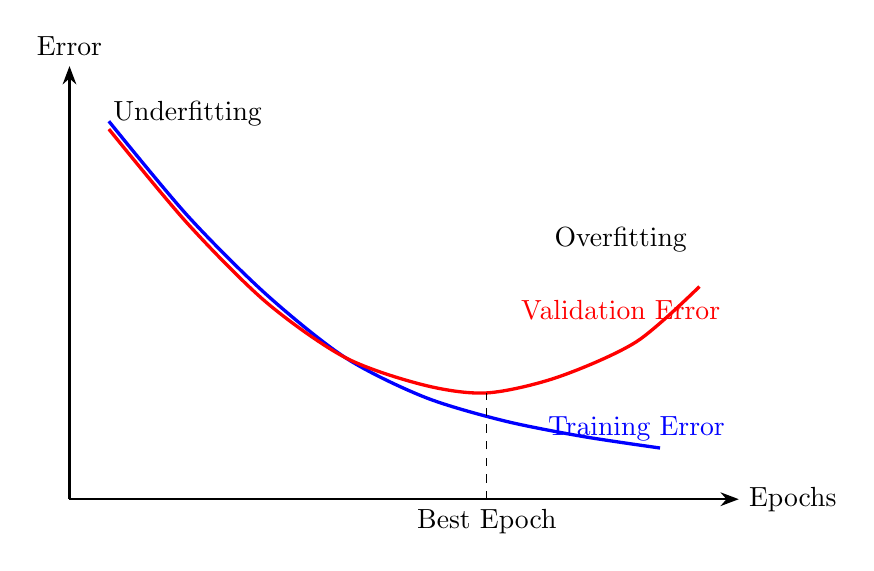
\begin{tikzpicture}[scale=1.0,>=Stealth]
		
		% Axes
		\draw[->,thick] (0,0)--(8.5,0) node[right]{Epochs};
		\draw[->,thick] (0,0)--(0,5.5) node[above]{Error};
		
		% Training curve
		\draw[very thick,blue]
		plot[smooth]
		coordinates{
			(0.5,4.8)
			(1.5,3.6)
			(2.5,2.6)
			(3.5,1.8)
			(4.5,1.3)
			(5.5,1.0)
			(6.5,0.8)
			(7.5,0.65)
		};
		
		% Validation curve
		\draw[very thick,red]
		plot[smooth]
		coordinates{
			(0.5,4.7)
			(1.5,3.5)
			(2.5,2.5)
			(3.5,1.8)
			(4.5,1.45)
			(5.3,1.35)
			(6.2,1.55)
			(7.2,2.0)
			(8.0,2.7)
		};
		
		% Best epoch
		\draw[dashed] (5.3,0)--(5.3,1.35);
		
		\node[below] at (5.3,0){Best Epoch};
		
		\node[blue] at (7.2,0.9){Training Error};
		
		\node[red] at (7.0,2.4){Validation Error};
		
		\node at (1.5,4.9){Underfitting};
		
		\node at (7.0,3.3){Overfitting};
		
	\end{tikzpicture}
\end{center}

%%%%%%%%%%%%%%%%%%%%%%%%%%%%%%%%%%%%%%%%%%%%%%%%%%%%%%%%%%%

\subsection{Why Early Stopping?}

The objective of early stopping is to stop training before the model
starts overfitting.

The best model is usually the one corresponding to the minimum validation
error rather than the minimum training error.

%%%%%%%%%%%%%%%%%%%%%%%%%%%%%%%%%%%%%%%%%%%%%%%%%%%%%%%%%%%

\section{Patience}

In practice, especially in deep learning, validation error may fluctuate
slightly from one epoch to another.

Therefore, instead of stopping immediately when validation error increases,
we introduce a parameter called \textbf{patience}.

\[
\boxed{
	\text{Patience}=
	\text{Number of epochs to wait after the last improvement in validation error.}
}
\]

%%%%%%%%%%%%%%%%%%%%%%%%%%%%%%%%%%%%%%%%%%%%%%%%%%%%%%%%%%%

\subsection{Example}

Suppose

\[
\text{Patience}=5.
\]

If the validation error does not improve for five consecutive epochs,
training stops even if the training error is still decreasing.

%%%%%%%%%%%%%%%%%%%%%%%%%%%%%%%%%%%%%%%%%%%%%%%%%%%%%%%%%%%

\subsection{Why Patience Matters}

\begin{itemize}
	
	\item \textbf{Patience Too Small}
	
	Training may stop too early due to temporary fluctuations in validation
	error.
	
	The resulting model may still be underfitting.
	
	\vspace{0.3cm}
	
	\item \textbf{Patience Too Large}
	
	Training continues for many unnecessary epochs.
	
	Although the training error keeps decreasing, the validation error may
	continue increasing, resulting in overfitting.
	
\end{itemize}

%%%%%%%%%%%%%%%%%%%%%%%%%%%%%%%%%%%%%%%%%%%%%%%%%%%%%%%%%%%

\section{Illustration of Patience}

\begin{center}
	\begin{tikzpicture}[scale=0.95,>=Stealth]
		
		% Axes
		\draw[->] (0,0)--(11,0) node[right]{Epoch};
		\draw[->] (0,0)--(0,5.5) node[above]{Validation Error};
		
		% Validation curve
		\draw[very thick,red]
		plot[smooth]
		coordinates{
			(0.5,5)
			(1.5,4)
			(2.5,3)
			(3.5,2.2)
			(4.5,1.5)
			(5.3,1.25)
			(6.2,1.35)
			(7.0,1.42)
			(8.0,1.50)
			(9.0,1.58)
			(10.0,1.68)
		};
		
		% Best model
		\fill (5.3,1.25) circle (2pt);
		
		\node[above] at (5.3,1.25){Best Model};
		
		\draw[dashed] (5.3,0)--(5.3,1.25);
		
		% Stop point
		\draw[dashed] (9.3,0)--(9.3,1.62);
		
		\node[below] at (9.3,0){Stop};
		
		\draw[<->]
		(5.3,-0.45)--(9.3,-0.45);
		
		\node at (7.3,-0.8){Patience = 4 epochs};
		
	\end{tikzpicture}
\end{center}

%%%%%%%%%%%%%%%%%%%%%%%%%%%%%%%%%%%%%%%%%%%%%%%%%%%%%%%%%%%

\section{Algorithm}

Suppose

\begin{itemize}
	\item Current epoch = $k$
	\item Patience = $P$
\end{itemize}

If there has been no improvement in validation error during the previous
$P$ epochs, then

\[
\boxed{
	\begin{aligned}
		\text{Stop Training}
		\quad\text{and}\quad
		\text{Restore the Model}\\
		\text{saved at epoch }(k-P).
	\end{aligned}
}
\]

%%%%%%%%%%%%%%%%%%%%%%%%%%%%%%%%%%%%%%%%%%%%%%%%%%%%%%%%%%%

\section*{Key Takeaways}

\begin{itemize}
	
	\item Training error continuously decreases during optimization.
	
	\item Validation error initially decreases but eventually increases due to overfitting.
	
	\item Early stopping selects the model corresponding to the minimum validation error.
	
	\item Patience prevents stopping because of temporary fluctuations in validation performance.
	
	\item A suitable patience value improves generalization while avoiding unnecessary training.
	
\end{itemize}

\section{Early Stopping as Regularization}

Early stopping is one of the simplest and most effective forms of
regularization in deep learning.

\begin{itemize}
	\item It is one of the most widely used regularization techniques.
	\item It can be used independently or together with other regularizers
	such as $L_2$ regularization, dropout, etc.
	\item It prevents the model parameters from growing excessively,
	thereby reducing overfitting.
\end{itemize}

%%%%%%%%%%%%%%%%%%%%%%%%%%%%%%%%%%%%%%%%%%%%%%%%%%%%%%%%%%%%%%

\subsection{Intuition}

Recall the SGD update rule

\[
\mathbf{w}_{t+1}
=
\mathbf{w}_{t}
-\eta \nabla L(\mathbf{w}_{t}),
\]

or equivalently,

\[
\mathbf{w}_{t}
=
\mathbf{w}_{0}
-
\eta
\sum_{i=1}^{t}
\nabla L(\mathbf{w}_{i-1}).
\]

Suppose

\[
\left\|
\nabla L(\mathbf{w})
\right\|
\le \tau,
\]

where $\tau$ is the maximum magnitude of the gradient.

Then,

\[
\|\mathbf{w}_{t}\|
\le
\|\mathbf{w}_{0}\|
+
\eta t\tau.
\]

Hence, the magnitude of the parameter vector can grow at most linearly
with the number of iterations.

Therefore, stopping training early prevents the weights from becoming
unnecessarily large.

%%%%%%%%%%%%%%%%%%%%%%%%%%%%%%%%%%%%%%%%%%%%%%%%%%%%%%%%%%%%%%

\subsection{Quadratic Approximation of the Loss}

Assume the loss is locally quadratic around its optimum
$\mathbf{w}^{*}$.

Using the second-order Taylor expansion,

\[
L(\mathbf{w})
=
L(\mathbf{w}^{*})
+
(\mathbf{w}-\mathbf{w}^{*})^{T}
\nabla L(\mathbf{w}^{*})
+
\frac12
(\mathbf{w}-\mathbf{w}^{*})^{T}
H
(\mathbf{w}-\mathbf{w}^{*}),
\]

where

\[
H
=
\nabla^{2}L(\mathbf{w}^{*})
\]

is the Hessian matrix.

Since

\[
\nabla L(\mathbf{w}^{*})=0,
\]

the approximation becomes

\[
L(\mathbf{w})
=
L(\mathbf{w}^{*})
+
\frac12
(\mathbf{w}-\mathbf{w}^{*})^{T}
H
(\mathbf{w}-\mathbf{w}^{*}).
\]

Differentiating,

\[
\nabla L(\mathbf{w})
=
H(\mathbf{w}-\mathbf{w}^{*}).
\]

%%%%%%%%%%%%%%%%%%%%%%%%%%%%%%%%%%%%%%%%%%%%%%%%%%%%%%%%%%%%%%

\subsection{SGD Update}

Substituting the gradient into SGD,

\[
\mathbf{w}_{t}
=
\mathbf{w}_{t-1}
-
\eta
H
(\mathbf{w}_{t-1}-\mathbf{w}^{*}).
\]

Rearranging,

\[
\boxed{
	\mathbf{w}_{t}
	=
	(I-\eta H)\mathbf{w}_{t-1}
	+
	\eta H\mathbf{w}^{*}.
}
\]

%%%%%%%%%%%%%%%%%%%%%%%%%%%%%%%%%%%%%%%%%%%%%%%%%%%%%%%%%%%%%%

\subsection{Eigenvalue Decomposition}

Let the Hessian have the eigendecomposition

\[
H
=
Q\Lambda Q^{T},
\]

where

\begin{itemize}
	\item $Q$ contains the orthonormal eigenvectors,
	\item $\Lambda=\operatorname{diag}(\lambda_1,\ldots,\lambda_n)$.
\end{itemize}

Then,

\[
\boxed{
	\mathbf{w}_{t}
	=
	(I-\eta Q\Lambda Q^{T})
	\mathbf{w}_{t-1}
	+
	\eta Q\Lambda Q^{T}\mathbf{w}^{*}.
}
\]

%%%%%%%%%%%%%%%%%%%%%%%%%%%%%%%%%%%%%%%%%%%%%%%%%%%%%%%%%%%%%%

\subsection{Solution}

Assume the initialization

\[
\mathbf{w}_0=\mathbf{0}.
\]

Then,

\[
\boxed{
	\mathbf{w}_{t}
	=
	Q
	\left[
	I-(I-\eta\Lambda)^t
	\right]
	Q^{T}
	\mathbf{w}^{*}.
}
\]

%%%%%%%%%%%%%%%%%%%%%%%%%%%%%%%%%%%%%%%%%%%%%%%%%%%%%%%%%%%%%%

\subsection{Connection with $L_2$ Regularization}

Recall the solution obtained using $L_2$ regularization,

\[
\boxed{
	\tilde{\mathbf{w}}
	=
	Q
	\left[
	I-(\Lambda+\alpha I)^{-1}\alpha
	\right]
	Q^{T}
	\mathbf{w}^{*}.
}
\]

Comparing the two expressions,

\[
(I-\eta\Lambda)^t
\approx
(\Lambda+\alpha I)^{-1}\alpha,
\]

shows that early stopping behaves similarly to
$L_2$ regularization.

Thus, early stopping is often viewed as an implicit form of
regularization.

%%%%%%%%%%%%%%%%%%%%%%%%%%%%%%%%%%%%%%%%%%%%%%%%%%%%%%%%%%%%%%

\section{Why Does Early Stopping Regularize?}

Early stopping allows only a limited number of parameter updates.

Suppose a parameter $w_i$ corresponds to an important direction of the
loss surface.

Then,

\[
\left|
\frac{\partial L}{\partial w_i}
\right|
\]

is relatively large, so the parameter receives larger updates and
converges quickly.

On the other hand, if

\[
\left|
\frac{\partial L}{\partial w_i}
\right|
\]

is small, then the parameter changes only slowly.

Since training is stopped before complete convergence, these parameters
never become excessively large.

Consequently,

\begin{itemize}
	\item parameters corresponding to important directions are learned,
	\item parameters corresponding to less important directions remain
	small,
	\item model complexity is reduced,
	\item overfitting is minimized.
\end{itemize}

%%%%%%%%%%%%%%%%%%%%%%%%%%%%%%%%%%%%%%%%%%%%%%%%%%%%%%%%%%%%%%

\subsection*{Key Takeaways}

\begin{enumerate}
	\item Early stopping is one of the most effective implicit regularization techniques.
	\item It limits the growth of model parameters by restricting the number of SGD updates.
	\item Under a quadratic approximation of the loss, early stopping behaves similarly to $L_2$ regularization.
	\item Important parameters converge rapidly, whereas less important parameters remain small.
	\item The resulting model usually generalizes better to unseen data.
\end{enumerate}

%################# Ensemble Method#############################
%%%%%%%%%%%%%%%%%%%%%%%%%%%%%%%%%%%%%%%%%%%%%%%%%%%%%%%%%%%%%%%%%%
\section{Ensemble Methods}

An \textbf{Ensemble Method} combines the predictions of multiple machine
learning models to obtain a more accurate and robust final prediction.

The individual models can be

\begin{itemize}
	\item Different learning algorithms
	(Logistic Regression, SVM, Decision Tree, Neural Network, etc.)
	\item Different instances of the same learning algorithm.
\end{itemize}

The individual models are typically trained using

\begin{itemize}
	\item Different hyperparameters,
	\item Different subsets of features,
	\item Different subsets of training samples.
\end{itemize}

%%%%%%%%%%%%%%%%%%%%%%%%%%%%%%%%%%%%%%%%%%%%%%%%%%%%%%%%%%%%%%%%%%
\subsection{Architecture}

\begin{center}
	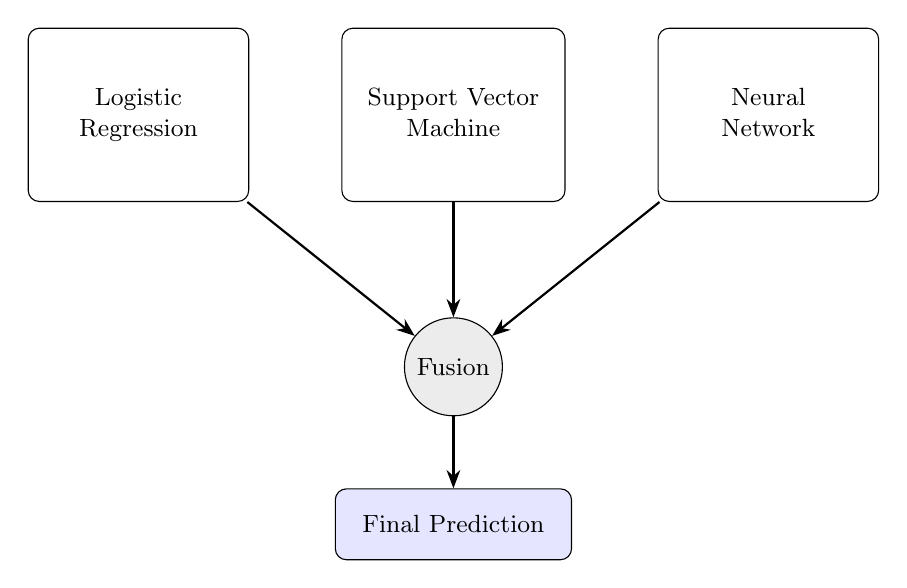
\begin{tikzpicture}[>=Stealth,
		every node/.style={font=\small},
		model/.style={draw,rounded corners,minimum width=2.8cm,minimum height=2.2cm},
		fusion/.style={draw,circle,minimum size=9mm,fill=gray!15},
		]
		
		% Models
		\node[model] (lr) at (0,0)
		{
			\begin{tabular}{c}
				Logistic\\Regression
			\end{tabular}
		};
		
		\node[model] (svm) at (4,0)
		{
			\begin{tabular}{c}
				Support Vector\\Machine
			\end{tabular}
		};
		
		\node[model] (nn) at (8,0)
		{
			\begin{tabular}{c}
				Neural\\Network
			\end{tabular}
		};
		
		% Fusion node
		\node[fusion] (f) at (4,-3.2) {Fusion};
		
		\node[draw,rounded corners,fill=blue!10,
		minimum width=3cm,minimum height=0.9cm]
		(out) at (4,-5.2)
		{Final Prediction};
		
		\draw[->,thick] (lr)--(f);
		\draw[->,thick] (svm)--(f);
		\draw[->,thick] (nn)--(f);
		
		\draw[->,thick] (f)--(out);
		
	\end{tikzpicture}
\end{center}

The outputs of all base learners are combined using an aggregation rule
such as

\[
\text{Average},\qquad
\text{Majority Voting},\qquad
\text{Weighted Average}.
\]

%%%%%%%%%%%%%%%%%%%%%%%%%%%%%%%%%%%%%%%%%%%%%%%%%%%%%%%%%%%%%%%%%%
\section{Bagging}

Bagging stands for

\[
\boxed{\textbf{Bootstrap Aggregating}}
\]

It is an ensemble technique in which

\begin{enumerate}
	\item Multiple bootstrap datasets are created from the original training data.
	\item A separate classifier is trained on each bootstrap sample.
	\item The predictions of all classifiers are combined to obtain the final prediction.
\end{enumerate}

%%%%%%%%%%%%%%%%%%%%%%%%%%%%%%%%%%%%%%%%%%%%%%%%%%%%%%%%%%%%%%%%%%
\subsection{Why Does Bagging Work?}

Suppose there are $k$ classifiers.

Each classifier produces an error

\[
e_i.
\]

Assume

\[
E[e_i]=0,
\]

and

\[
\operatorname{Var}(e_i)=V.
\]

Further,

\[
\operatorname{Cov}(e_i,e_j)=C,
\qquad i\neq j.
\]

%%%%%%%%%%%%%%%%%%%%%%%%%%%%%%%%%%%%%%%%%%%%%%%%%%%%%%%%%%%%%%%%%%
\subsection{Average Prediction Error}

The ensemble prediction error is

\[
\bar e
=
\frac1k
\sum_{i=1}^{k}
e_i.
\]

The mean squared error is

\[
MSE
=
E[\bar e^2].
\]

Substituting,

\[
=
E
\left[
\left(
\frac1k
\sum_{i=1}^{k}
e_i
\right)^2
\right].
\]

Expanding,

\[
=
\frac1{k^2}
E
\left[
\sum_i e_i^2
+
\sum_{i\neq j}
e_ie_j
\right].
\]

Using

\[
E[e_i^2]=V,
\]

and

\[
E[e_ie_j]=C,
\]

we obtain

\[
=
\frac1{k^2}
\left[
kV
+
k(k-1)C
\right].
\]

Hence,

\[
\boxed{
	MSE
	=
	\frac{V}{k}
	+
	\frac{k-1}{k}C.
}
\]

%%%%%%%%%%%%%%%%%%%%%%%%%%%%%%%%%%%%%%%%%%%%%%%%%%%%%%%%%%%%%%%%%%
\section{Interpretation}

The ensemble error depends on two quantities:

\begin{enumerate}
	\item Variance of individual models ($V$)
	\item Correlation between their errors ($C$)
\end{enumerate}

%%%%%%%%%%%%%%%%%%%%%%%%%%%%%%%%%%%%%%%%%%%%%%%%%%%%%%%%%%%%%%%%%%
\subsection*{Case 1: Independent Errors}

If the individual models are independent,

\[
C=0,
\]

then

\[
\boxed{
	MSE=\frac{V}{k}.
}
\]

Therefore,

\[
\boxed{
	\text{Increasing the number of models reduces the error.}
}
\]

%%%%%%%%%%%%%%%%%%%%%%%%%%%%%%%%%%%%%%%%%%%%%%%%%%%%%%%%%%%%%%%%%%
\subsection*{Case 2: Perfectly Correlated Errors}

If every model makes exactly the same mistakes,

\[
C=V,
\]

then

\[
MSE
=
\frac{V}{k}
+
\frac{k-1}{k}V
=
V.
\]

Hence,

\[
\boxed{
	\text{No improvement is obtained by bagging.}
}
\]

%%%%%%%%%%%%%%%%%%%%%%%%%%%%%%%%%%%%%%%%%%%%%%%%%%%%%%%%%%%%%%%%%%
\subsection*{Conclusion}

Bagging is effective only when the individual models make
different (uncorrelated) errors.

Therefore,

\[
\boxed{
	\text{Lower correlation among models}
	\Longrightarrow
	\text{Greater improvement from ensemble learning.}
}
\]

%%%%%%%%%%%%%%%%%%%%%%%%%%%%%%%%%%%%%%%%%%%%%%%%%%%%%%%%%%%%%%%%%%
\section*{Key Points}

\begin{itemize}
	\item Ensemble methods combine multiple models.
	\item Diversity among models is essential.
	\item Bagging reduces variance.
	\item Independent errors provide maximum reduction in prediction error.
	\item Highly correlated models offer little benefit.
\end{itemize}



%################## Dropout##############################







\end{document}